Este capítulo detalla el desarrollo técnico y la programación de los componentes principales de \textit{Reset}. A lo largo de las siguientes secciones se explica la arquitectura del código y el funcionamiento de los sistemas creados a medida, como los gestores globales de guardado y diálogos, las físicas de movimiento del personaje y el comportamiento de la inteligencia artificial de los enemigos en cada mundo.

% =========================================================================
\section{Arquitectura del Sistema y Persistencia Global}
\label{sec:arquitectura_gestores}
El pilar estructural de \textit{Reset} es su sistema de gestores globales unificados bajo la jerarquía del \textit{Game Object} persistente \texttt{Global\_Managers}, el cual se mantiene activo entre cargas de escenas mediante la instrucción \texttt{DontDestroyOnLoad()}. Estos componentes operan bajo el patrón de diseño \textit{Singleton}, proporcionando un punto de acceso centralizado y seguro para el control de la persistencia de datos, la gestión de audio y el flujo de los diálogos.

Para garantizar que solo exista una instancia activa de cada gestor en memoria y evitar duplicados al recargar el Hub, se programó la siguiente lógica de inicialización en el despertar del script:

\begin{verbatim}
public static SaveManager Instance { get; private set; }

private void Awake()
{
    if (Instance != null && Instance != this)
    {
        Destroy(gameObject);
        return;
    }
    Instance = this;
    DontDestroyOnLoad(gameObject);
}
\end{verbatim}

\subsection{Sistema de Persistencia y Guardado de Datos (\texttt{SaveManager.cs})}
El sistema de persistencia de datos se enfrenta a un reto de diseño clásico en Unity: la imposibilidad de serializar directamente a formato de disco (\texttt{JSON} o bases de datos) referencias en memoria a objetos complejos de la escena, como prefabricados (\textit{Prefabs}) o el estado físico de los enemigos. 

Para resolver este acoplamiento técnico y organizar la persistencia del proyecto, el sistema se ha estructurado en tres bloques lógicos de guardado detallados como se aprecia en la Figura~\ref{fig:singletonsavemanager}:

\begin{figure}[H]
    \centering
    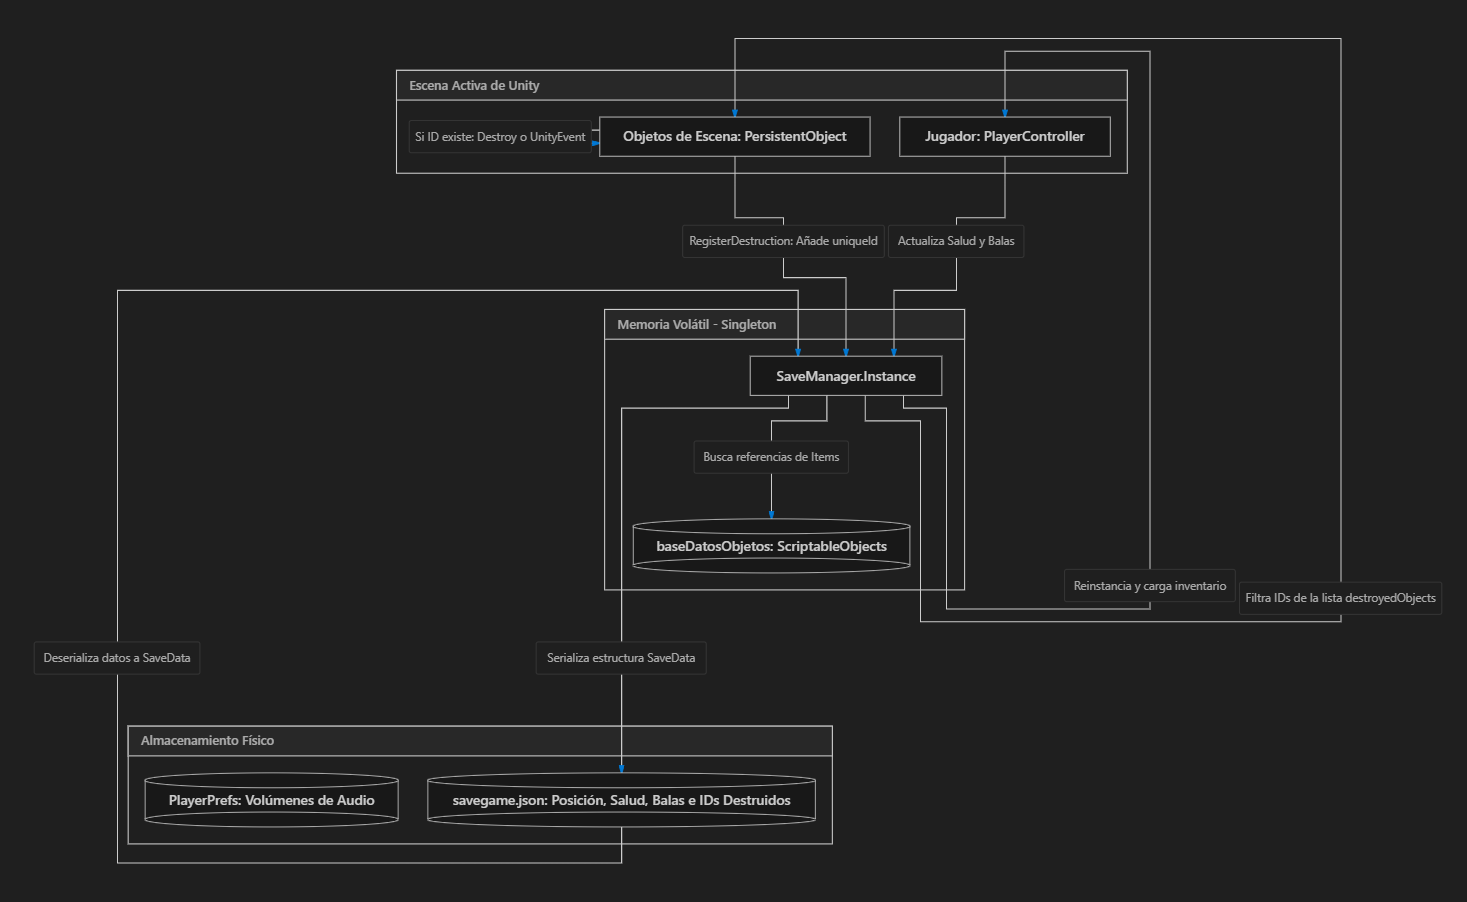
\includegraphics[width=\textwidth]{pages/img/SingletonSaveManager.png}
    \caption{Patrón Singleton del \texttt{SaveManager}.}
    \label{fig:singletonsavemanager}
\end{figure}

\begin{enumerate}
    \item \textbf{Configuración Global y Opciones de Sonido:} 
    Las opciones de configuración (como los niveles de volumen de la música y los efectos de sonido) se gestionan de forma de persistencia global. Dado que estos parámetros deben ser independientes de la partida o del nivel activo (deben conservarse incluso si el jugador pulsa ``Nueva Partida''), se guardan directamente en el registro del sistema mediante la clase nativa \texttt{PlayerPrefs} de Unity.
    
    \item \textbf{Estadísticas y Posición del Jugador:}
    Los datos dinámicos del avatar y el progreso se gestionan a través de la estructura serializable \texttt{SaveData}, que se escribe en un archivo JSON en disco (\texttt{savegame.json}). En este bloque se guardan:
    \begin{itemize}
        \item La escena activa donde se encuentra el jugador.
        \item La posición exacta (coordenadas $X$ e $Y$) en el mapa.
        \item La salud actual y máxima del personaje.
        \item Las balas cargadas en el arma activa y las almacenadas en las ranuras de inventario.
        \item La lista de identificadores (\texttt{string ID}) del inventario. Al cargar, el gestor utiliza una base de datos estática de referencia cruzada que actúa bajo una filosofía similar al patrón de diseño \textit{Flyweight} (peso ligero): se almacenan referencias directas a todos los \texttt{ItemData} (\textit{ScriptableObjects}) estáticos del proyecto en una tabla de búsqueda en memoria (\texttt{baseDatosObjetos}), evitando serializar instancias pesadas en el JSON y cargando de forma dinámica solo los identificadores dinámicos que el jugador posee en su sesión.
    \end{itemize}

    \item \textbf{Objetos Persistentes del Escenario y Enemigos (\texttt{PersistentObject.cs}):}
    Para guardar si una caja rompible ya se ha destruido, si un enemigo ha sido derrotado o si un trigger ya se ha activado, se desarrolló el script modular \texttt{PersistentObject.cs}. Este componente se añade a cualquier objeto de la escena que deba recordar su estado y funciona de la siguiente manera:
    \begin{itemize}
        \item \textit{Autogeneración de Identificadores Únicos:} El script autogenera un código único combinando el nombre de la escena, el nombre del objeto y sus coordenadas espaciales aproximadas con dos decimales de precisión:
\begin{verbatim}
uniqueId = $"{sceneName}_{gameObject.name}_" +
           $"{transform.position.x:F2}_{transform.position.y:F2}";
\end{verbatim}
        Esto garantiza IDs únicos de forma automática para todos los objetos del mapa sin tener que escribirlos uno a uno a mano.
        \item \textit{Registro de Destrucción:} Cuando una caja se rompe o un enemigo muere, se llama al método \texttt{RegisterDestruction()}, que añade su \texttt{uniqueId} a la lista de objetos destruidos del \texttt{SaveManager}.
        \item \textit{Carga Condicional:} Al iniciar la escena, el script comprueba si su ID ya figura en la lista de destruidos. Si la variable \texttt{destroyOnLoad} es verdadera, el objeto se autodestruye de inmediato (\texttt{Destroy(gameObject)}). Si es falsa, invoca el evento \texttt{onAlreadyTriggered} (un \texttt{UnityEvent}) para ejecutar acciones alternativas, como mantener una compuerta abierta o un botón pulsado.
    \end{itemize}
\end{enumerate}

El guardado físico de la estructura \texttt{SaveData} y de la lista de IDs destruidos se escribe en un archivo JSON ubicado en la ruta persistente del sistema operativo (ver Figura~\ref{fig:singletonsavemanager}) mediante la llamada:
\begin{verbatim}
saveFilePath = Path.Combine(Application.persistentDataPath, "savegame.json");
\end{verbatim}

\subsubsection{Lógica de Flujo de Transiciones y Gestión de Muerte en Mundo 1}
El gestor del guardado implementa tres rutinas fundamentales para salvaguardar el estado de la simulación:
\begin{itemize}
    \item \textbf{Carga Priorizada sobre Disco:} Al realizar una transición entre niveles o volver al Hub, el gestor lee los datos desde el almacenamiento físico local si detecta que la escena de destino coincide con el registro del archivo JSON. Esto evita inconsistencias de datos, impidiendo que el inventario o la salud del avatar se corrompan si el jugador altera el flujo de la partida.
    \item \textbf{Control de Muerte y Reinicios Limpios:} Si la salud del jugador llega a cero, el juego ejecuta una evaluación condicional:
    \begin{itemize}
        \item \textit{Caso Sin Guardado:} Si el usuario no ha guardado partida de forma voluntaria en el nivel actual a través del menú de pausa, el método \texttt{RestaurarEstadoPorDefecto()} limpia las listas de persistencia en memoria y vacía el inventario. Esto provoca que al recargar la escena, todos los enemigos, cajas rompibles y tarjetas de misión vuelvan a instanciarse por defecto.
        \item \textit{Caso Con Guardado:} Si existe un archivo \texttt{savegame.json} en disco, el método lee la posición del jugador, su salud actual, su munición exacta y la lista de IDs de objetos marcados como destruidos. Al reconstruir el nivel, el script destruye preventivamente del mapa cualquier caja o tarjeta que el jugador ya hubiese recogido en su sesión guardada.
    \end{itemize}
    \item \textbf{Pantalla de Nueva Partida y Limpieza:} El método \texttt{DeleteSaveGame()} elimina físicamente el archivo JSON y limpia los registros de sistema (\texttt{PlayerPrefs}) que controlan la validación de finalización de niveles (ej. \texttt{LevelCompleted\_1\_Level1}). Esto garantiza que al pulsar ``Nueva Partida'' los portales del Hub inician en su estado original bloqueado.
\end{itemize}

\subsection{Sistema de Diálogos y Eventos Narrativos}
Para gestionar las interacciones narrativas de forma modular y desacoplada, se ha diseñado y programado un \textbf{sistema de diálogos de desarrollo propio al $100\%$}, evitando el uso de herramientas o complementos externos de terceros. La representación visual del sistema se implementa exclusivamente mediante los \textbf{componentes nativos y básicos de la interfaz de usuario de Unity (\textit{Canvas})}, empleando paneles gráficos estándar y dos contenedores de texto (\textit{TextMeshPro}) para mostrar dinámicamente el nombre del interlocutor y la frase activa. Este sistema se estructura sobre tres componentes lógicos principales: el gestor central (\texttt{DialogueManager.cs}), el disparador por interacción (\texttt{NPCDialogue.cs}) y el disparador por zona de colisión (\texttt{TriggerDialogue.cs}), los cuales se describen a continuación:

\subsubsection{1. Clases de Datos Serializables}
La información de las conversaciones se almacena en dos clases contenedoras marcadas con el atributo \texttt{[System.Serializable]} de Unity para permitir su edición directa en el editor:
\begin{itemize}
    \item \texttt{DialogueLine}: Contiene el nombre del emisor (\texttt{npcName}) y el texto de su frase (\texttt{sentence}). En el Inspector, el texto utiliza el decorador \texttt{[TextArea(3, 10)]} para habilitar un cuadro de edición multilínea cómodo para el diseñador.
    \item \texttt{Dialogue}: Contenedor que almacena una lista ordenada de tipo \texttt{DialogueLine} formando la conversación secuencial.
\end{itemize}

\subsubsection{2. El Motor de Diálogos (\texttt{DialogueManager.cs})}
Es el encargado de procesar la lógica de visualización y renderizado en pantalla. Funciona como un \textit{Singleton} global y realiza las siguientes operaciones:
\begin{itemize}
    \item \textit{Cola de Diálogo:} Al recibir una conversación, inicializa una cola de tipo FIFO (\textit{First In, First Out}) mediante la clase \texttt{Queue<DialogueLine>}, almacenando en ella todas las frases en orden secuencial.
    \item \textit{Control de Interfaz (UI):} Activa el panel de diálogo y actualiza dinámicamente los campos de texto (\texttt{TextMeshProUGUI}) destinados al nombre del hablante y a la frase actual.
    \item \textit{Efecto de Escritura (Typing Effect):} Mediante una corrutina de C\#, escribe la frase carácter a carácter con un desfase temporal regulado por una velocidad ajustable (\texttt{typingSpeed = 0.02f}). La implementación de este efecto mediante programación asíncrona por corrutinas permite distribuir la carga computacional a lo largo de varios fotogramas, evitando el bloqueo del hilo principal de ejecución (\textit{Main Thread}) y garantizando la fluidez de la simulación:
\end{itemize}
\begin{verbatim}
private IEnumerator TypeSentence(string sentence)
{
    dialogueText.text = "";
    isTyping = true;
    foreach (char letter in sentence.ToCharArray())
    {
        dialogueText.text += letter;
        yield return new WaitForSeconds(typingSpeed);
    }
    isTyping = false;
}
\end{verbatim}
\begin{itemize}
    \item \textit{Callbacks de Finalización:} Al vaciarse la cola de frases, el gestor oculta la interfaz y ejecuta una acción de retorno (\texttt{System.Action}), permitiendo a otros scripts reaccionar cuando un diálogo termina.
\end{itemize}

\subsubsection{3. Disparador por Interacción de Personaje (\texttt{NPCDialogue.cs})}
Este script se asocia a los personajes no jugables (NPC) con los que el jugador puede interactuar voluntariamente pulsando la tecla de acción. 
\begin{itemize}
    \item Contiene los datos de la conversación en una variable de tipo \texttt{Dialogue}.
    \item Llama al gestor pasándole un callback que, al finalizar el diálogo, invoca un evento local de Unity (\texttt{UnityEvent alTerminarDialogo}). Esta implementación responde al patrón de diseño \textit{Observer} (observador), desacoplando por completo el motor de diálogos global de las repercusiones lógicas locales en la escena (como abrir compuertas o spawnear objetos físicos).
\end{itemize}

\subsubsection{4. Disparador por Zona de Colisión (\texttt{TriggerDialogue.cs})}
Se utiliza para diálogos que deben saltar de forma automática cuando el jugador pisa un área invisible del mapa (\texttt{OnTriggerEnter2D}):
\begin{itemize}
    \item \textit{Condición de Progreso:} Permite establecer un requisito de núcleos necesarios mediante la variable \texttt{coresRequeridos} (por ejemplo, el diálogo solo se activa si el jugador posee exactamente 3 núcleos).
    \item \textit{Persistencia ante Cargas:} Asocia un identificador único opcional (\texttt{dialogoID}). Al completarse la conversación, este ID se añade a la lista de diálogos reproducidos de la partida en el \texttt{SaveManager}. Al iniciar la escena, si el ID ya figura en dicha lista, el trigger se destruye de inmediato (\texttt{Destroy(gameObject)}) para evitar que la escena cinemática o el diálogo se repitan al volver a cargar el nivel.
\end{itemize}

\subsection{Iluminación Dinámica (\texttt{FlickerLight2D.cs})}
Para dotar al menú principal de una ambientación retro coherente con la temática, se diseñó un algoritmo de parpadeo aleatorio para el componente \texttt{Light2D} del motor gráfico universal (URP) de Unity. El script simula el parpadeo de una pantalla rota de las clasicas pantallas antiguas de televisión (ver Figura~\ref{fig:mainmenureset}), esto ocurre calculando fluctuaciones aleatorias de intensidad tamizadas por rangos mínimos y máximos:
\begin{verbatim}
private IEnumerator FlickerRoutine()
{
    while (true)
    {
        targetLight.intensity = Random.Range(minIntensity, maxIntensity);
        float delay = Random.Range(minFlickerSpeed, maxFlickerSpeed);
        yield return new WaitForSeconds(delay);
    }
}
\end{verbatim}

\begin{figure}[H]
    \centering
    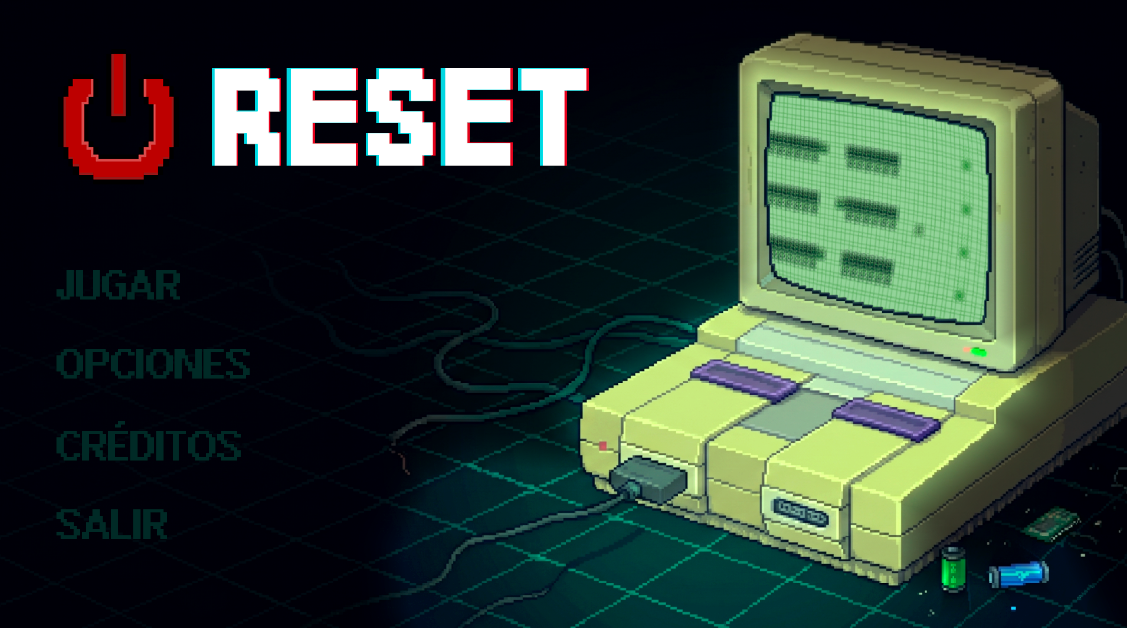
\includegraphics[width=0.75\textwidth]{pages/img/MainMenuReset.png}
    \caption{Menú principal con estética retro de \textit{Reset}.}
    \label{fig:mainmenureset}
\end{figure}

Asimismo, este script fue adaptado para su uso en el menú de selección de niveles del Mundo 1. En dicha interfaz, la lógica de parpadeo se configuró con parámetros de oscilación mucho más sutiles y progresivos con el fin de emular la icónica estética del menú principal de \textit{The Last of Us} (ver Figura~\ref{fig:tlrmenu}). El sistema de iluminación ambiental recrea visualmente una ventana donde la luz exterior incide y fluctúa de forma tenue en lugar de una interferencia eléctrica, lo que contribuye de manera notable a la inmersión y ambientación del jugador desde la navegación por las interfaces.

% =========================================================================
\section{Mundo 1: Mecánicas Cenitales y Algoritmos de Inteligencia Artificial}
\label{sec:mecanicas_mundo1_tecnico}
El primer plano de juego (Mundo 1) utiliza una perspectiva cenital (\textit{Top-Down}). En este entorno, el reto de desarrollo principal consistió en dotar a los enemigos infectados de una inteligencia táctica y un comportamiento orgánico de persecución y huida.

\subsection{Navegación Táctica por Direccionamiento de Contexto (Context Steering)}
Para resolver la navegación local y la evitación de obstáculos dinámica de los infectados, se ha prescindido de los sistemas estándar de Unity basados en mallas de navegación. En su lugar, se implementó un sistema de \textbf{Context Steering} (direccionamiento por contexto) en dos dimensiones.
El algoritmo opera en base a un círculo de 8 vectores de dirección predefinidos ($\vec{d}_i$ para $i = 0 \dots 7$, distribuidos cada $45^\circ$):
\begin{equation}
\vec{d}_0 = (0, 1), \, \vec{d}_1 = (0.7, 0.7), \, \vec{d}_2 = (1, 0), \, \dots
\end{equation}

\begin{figure}[H]
    \centering
    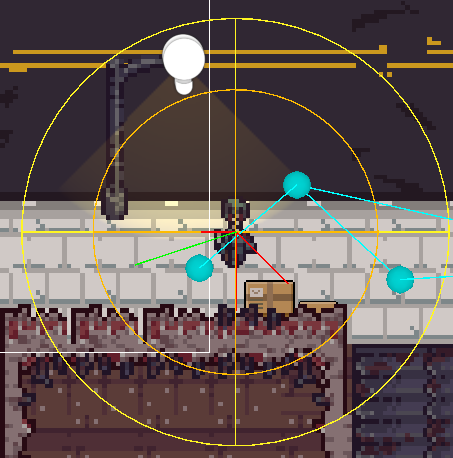
\includegraphics[width=0.45\textwidth]{pages/img/ContextSteering.png}
    \caption{Context Steering visual.}
    \label{fig:contextsteering}
\end{figure}

En cada paso físico de simulación (\texttt{FixedUpdate}), el enemigo ejecuta tres fases de cálculo (como se aprecia en la Figura~\ref{fig:contextsteering}):

\subsubsection{1. Fase de Interés}
Se calcula un array de valores de interés ($I_i$) que mide cómo de alineada está cada una de las 8 direcciones con respecto al vector de dirección normalizado que apunta al objetivo ($\vec{d}_{obj}$). Esta alineación se obtiene mediante el producto escalar entre vectores, descartando los valores negativos que representan direcciones opuestas al objetivo:
\begin{equation}
I_i = \max(0, \, \vec{d}_i \cdot \vec{d}_{obj})
\end{equation}
\subsubsection{2. Fase de Peligro}
Se calcula un array de valores de peligro ($D_i$) para cada una de las direcciones. El script proyecta un haz circular físico (\texttt{Physics2D.CircleCast}) con un radio de colisión del enemigo ($r_{enemigo} = 0.4$) hasta una distancia máxima de detección ($L_{raycast} = 1.0$) en la capa de colisiones del mapa. Si hay impacto con un obstáculo físico, el valor del peligro se pondera según la cercanía del punto de colisión:
\begin{equation}
D_i = \begin{cases} 
1 - \left( \frac{d_{impacto}}{L_{raycast}} \right) & \mbox{si colisiona} \\ 
0 & \mbox{si no colisiona} 
\end{cases}
\end{equation}
Esto produce un valor numérico continuo entre $0$ (camino despejado) y $1$ (colisión inminente).
\subsubsection{3. Fusión Vectorial (Vector Blend)}
Se calcula la puntuación final de cada eje ($S_i$) restando el peligro ponderado por un factor de evasión ($\beta = 1.5$) que determina la agresividad con la que el enemigo esquiva los muros:
\begin{equation}
S_i = \max(0, \, I_i - D_i \cdot \beta)
\end{equation}
El vector de movimiento resultante final ($\vec{v}_{final}$) se obtiene mediante la suma ponderada de todas las direcciones multiplicadas por su puntuación, normalizando el resultado final si es distinto de cero para mantener una velocidad lineal constante:
\begin{equation}
\vec{v}_{final} = \begin{cases}
\mbox{normalize}\left(\sum_{i=0}^{7} \vec{d}_i \cdot S_i\right) & \mbox{si } \sum S_i > 0 \\
\vec{d}_{obj} & \mbox{en caso de bloqueo absoluto}
\end{cases}
\end{equation}
Este proceso de fusión equilibra en tiempo real la atracción hacia el objetivo (vectores verdes) y la repulsión de las colisiones (vectores rojos) ilustradas en la Figura~\ref{fig:contextsteering}, resultando en una navegación fluida alrededor de obstáculos físicos.

\subsection{Comportamiento Físico y Movimiento Orgánico de los Zombies}
La inteligencia de los enemigos cenitales se gobierna mediante una Máquina de Estados Finitos (FSM) estructurada como una máquina de estados basada en enumerados que define cuatro estados de comportamiento lógico (ver Figura~\ref{fig:fsmenemigos}):
\begin{itemize}
    \item \textbf{\texttt{Patrullando}:} Movimiento pasivo a velocidad de patrulla entre los nodos designados en la jerarquía (\textit{Way Points}).
    \item \textbf{\texttt{Persiguiendo}:} Alerta activa que se dispara si el jugador entra en su rango de visión y existe una línea de visión directa libre de muros.
    \item \textbf{\texttt{Atacando}:} Estado de detención física y ejecución de la secuencia de daño por proximidad al jugador.
    \item \textbf{\texttt{Regresando}:} Si el jugador supera la distancia de pérdida de alerta, el enemigo se desplaza de vuelta a su zona de inicio.
\end{itemize}

\begin{figure}[H]
    \centering
    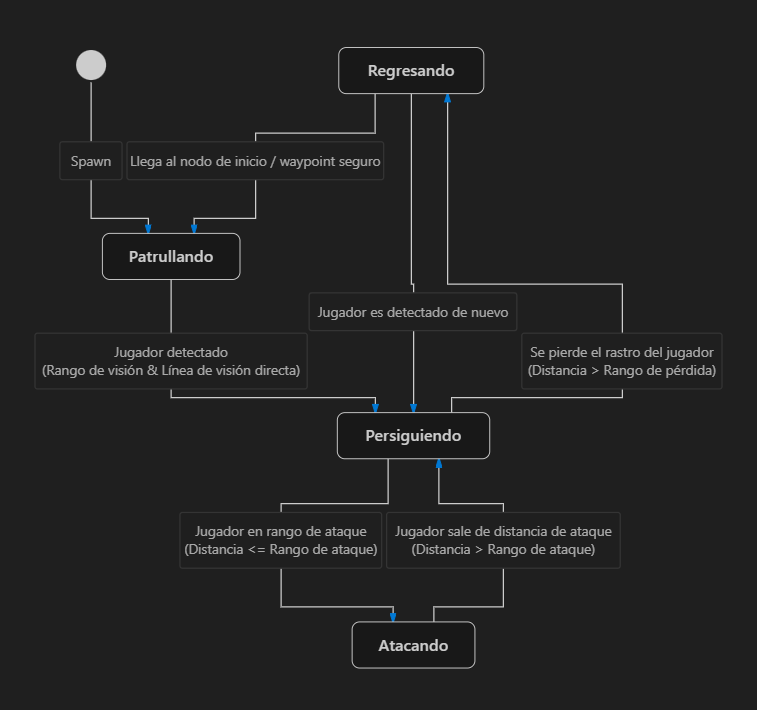
\includegraphics[width=0.75\textwidth]{pages/img/FSMEnemigos.png}
    \caption{Máquina de Estados Finitos (FSM) de los enemigos.}
    \label{fig:fsmenemigos}
\end{figure}

Para evitar que los zombies muestren desplazamientos lineales rígidos, se programó un comportamiento físico que inyecta ruido procedimental sinusoidal sobre los vectores de movimiento:

\subsubsection{Fase 1: Tambaleo o Movimiento Errático}
Se aplica de forma continua en patrulla y persecución. El script calcula una dirección perpendicular a la trayectoria actual del zombi:
\begin{equation}
\vec{d}_{perp} = (-v_y, \, v_x)
\end{equation}
A continuación, se aplica una oscilación sinusoidal basada en el tiempo del motor, sumando un valor de fase aleatorio ($\phi_{offset}$) al instanciarse en la escena, asegurando que las hordas no se balanceen de forma sincronizada:
\begin{equation}
f_{tambaleo} = \sin((t_{ejecucion} + \phi_{offset}) \cdot \omega_{tambaleo}) \cdot A_{amplitud}
\end{equation}
La dirección final de avance se modifica de la siguiente forma antes de aplicar la velocidad física al Rigidbody:
\begin{equation}
\vec{d}_{final} = \mbox{normalize}(\vec{d}_{final} + \vec{d}_{perp} \cdot f_{tambaleo})
\end{equation}
Esto inyecta un movimiento de balanceo lateral en zig-zag que emula de forma orgánica el caminar de un infectado clásico.

\subsubsection{Fase 2: Pasos Rápidos Probabilísticos}
Para simular brotes de agresividad durante la persecución a distancia media, se implementó una probabilidad de sprint por fotograma físico. A menos que esté en estado de frenesí cercano, el zombi evalúa de forma probabilística si acelera:
\begin{equation}
P(\mbox{sprint}) = p_{sprint} \cdot \Delta t_{physics}
\end{equation}
Si el número aleatorio es inferior a este umbral, el zombi activa un multiplicador de velocidad de paso rápido ($\times 2$) durante una ventana fija de $0.5$ segundos, simulando una pequeña zancada frenética hacia el jugador.

\subsubsection{Fase 3: Estado de Frenesí Cercano}
Si el jugador se encuentra a una distancia crítica menor o igual a la establecida, el enemigo ignora el paso rápido probabilístico y activa una infraestructura de velocidad de frenesí constante que multiplica su velocidad base por $1.5$, aumentando la tensión del jugador en el combate a corta distancia.

\subsection{El Algoritmo de Huida Táctica de los Enemigos a Distancia (Nivel 2)}
En el Nivel 2 de Mundo 1, los enemigos de disparo (\texttt{EnemyShooter.cs}), debido a que no poseen un comportamiento de patrulla, aplican un comportamiento espacial inverso para defender su rol de unidades de disparo a distancia. El script divide su zona de alerta en tres radios concéntricos respecto al jugador:
\begin{itemize}
    \item \textbf{Zona de Huida:} Si el jugador se aproxima demasiado, el zombi calcula un vector de escape opuesto aplicando una fuerza de escape dinámica (\textit{Flee Steering Behavior}):
    \begin{equation}
    \vec{d}_{huida} = \mbox{normalize}(\vec{x}_{zombi} - \vec{x}_{jugador})
    \end{equation}
    A continuación, establece como objetivo un punto situado en la dirección de escape y ejecuta el algoritmo de Context Steering hacia dicho objetivo, huyendo del jugador mientras esquiva muros en tiempo real.
    \item \textbf{Zona de Disparo Óptima:} El zombi anula su velocidad y dispara proyectiles con una cadencia fija, manteniendo su posición de combate.
    \item \textbf{Zona de Acercamiento:} El zombi avanza en dirección al jugador utilizando el Context Steering para acortar la distancia hasta entrar en el rango de tiro.
\end{itemize}

\subsection{Sistema Anti-atasco por Teleportación Recuperativa}
Para mitigar la ausencia de un mapa de nodos rígido y evitar atascos permanentes en esquinas cerradas del mapa, se diseñó un módulo de seguridad de detección de bloqueos espaciales (\textit{Deadlock Detection}). El script registra la posición del enemigo cada frame. Si la distancia recorrida con respecto a un punto de muestreo es inferior a un umbral mínimo de seguridad ($0.5$ metros) de forma ininterrumpida durante $3$ segundos de física en persecución, se incrementa el contador de atasco. 
Al alcanzar el límite, el enemigo anula sus fuerzas físicas, se teleporta de manera instantánea a las coordenadas del último nodo de patrulla seguro registrado en su memoria de ruta y devuelve su estado en la FSM a patrulla básica. Esto libera los recursos del Rigidbody y evita bloqueos en el flujo del nivel.

\subsection{Director de Drops y Ajuste de Dificultad Dinámico (DDA)}
Para regular la tensión, se programó un sistema en \texttt{ObjetoRompible.cs} que actúa como un Director de Recursos en base a un algoritmo de selección aleatoria ponderada (\textit{Weighted Random Selector}) alimentado por dos estadísticas del jugador: el ratio de salud actual ($H_{\%}$) y la cantidad de munición física restante ($A_{total}$). El sistema utiliza la matriz probabilística descrita en la Tabla~\ref{tab:drop_director} para recalcular las opciones de botín en tiempo real. Tras sumar los pesos de probabilidad dinámicos calculados, el método \texttt{ElegirDrop()} realiza la selección física del objeto que se va a instanciar en la escena mediante la sustracción sucesiva de rangos:

\begin{table}[htbp]
\centering
\resizebox{\textwidth}{!}{
    \begin{tabular}{|l|c|c|c|c|}
    \hline
    \textbf{Estado del Jugador} & \textbf{Peso Vendas ($W_v$)} & \textbf{Peso Botiquín ($W_b$)} & \textbf{Peso Balas ($W_m$)} & \textbf{Peso Nada ($W_n$)} \\ \hline
    $H_{\%} \ge 90\% \quad A_{total} \ge 15$ & 10 & 5 & 10 & 75 \\ \hline
    $H_{\%} \ge 90\% \quad A_{total} < 15$ & 15 & 5 & 30 & 50 \\ \hline
    $H_{\%} \le 35\% \quad A_{total} \ge 15$ & 50 & 35 & 0 & 15 \\ \hline
    $H_{\%} \le 35\% \quad A_{total} < 15$ & 50 & 30 & 10 & 10 \\ \hline
    Neutro / Estándar & 50 & 15 & 20 & 15 \\ \hline
    \end{tabular}
}
\caption{Matriz de pesos probabilísticos del Director de Drops en base al estado del jugador.}
\label{tab:drop_director}
\end{table}

\begin{verbatim}
private GameObject ElegirDrop(int pesoVendas, int pesoBotiquin,
                              int pesoBalas, int pesoNada)
{
    int totalPeso = pesoVendas + pesoBotiquin + pesoBalas + pesoNada;
    int rng = Random.Range(0, totalPeso);

    if (rng < pesoVendas) return prefabVendas;
    rng -= pesoVendas;

    if (rng < pesoBotiquin) return prefabBotiquin;
    rng -= pesoBotiquin;

    if (rng < pesoBalas) return prefabBalas;

    return null; // Nada
}
\end{verbatim}

Este algoritmo implementa un ajuste dinámico de dificultad (DDA), asegurando que un jugador hábil con abundancia de recursos reciba \textit{drops} vacíos (peso nada de $75$), mientras que un jugador en estado crítico reciba botiquines y vendas con un $85\%$ de probabilidad total, garantizando la supervivencia y la viabilidad del nivel.

% =========================================================================
\section{Mundo 2: Físicas de Plataformas e Interacción Aérea}
\label{sec:mecanicas_mundo2_tecnico}
El segundo mundo transiciona las físicas del motor al plano bidimensional lateral (\textit{Side-Scroller}) donde las sensaciones de salto y la inercia aérea son indispensables para asegurar el control del jugador.

\subsection{Ajustes de Física Fina y Mecánicas de Game Feel}
La implementación en el controlador físico refina el movimiento por defecto aplicando coeficientes de aceleración e inercia de la siguiente manera:
\begin{itemize}
    \item En el suelo, la aceleración y deceleración física se fijan en $45$ unidades, ofreciendo una respuesta instantánea al presionar o soltar el teclado.
    \item En el aire, para simular peso e inercia realistas, se reducen a $20$ y $15$ unidades respectivamente. Esto impide que el jugador cambie de dirección de forma inmediata en medio de un salto, obligándole a planificar sus trayectorias parabólicas.
\end{itemize}
Asimismo, se han programado tres algoritmos para el control del salto y compensación de la latencia de entrada (\textit{Input Latency}):

\begin{verbatim}
// Salto Variable
if (Input.GetButtonUp("Jump") && rb.linearVelocity.y > 0)
{
    rb.linearVelocity = new Vector2(rb.linearVelocity.x, 
                                    rb.linearVelocity.y * jumpHeightMultiplier);
}

// Estructura del Coyote Time y Jump Buffer
if (isGrounded)
{
    coyoteTimeCounter = coyoteTime;
}
else
{
    coyoteTimeCounter -= Time.deltaTime;
}

if (Input.GetButtonDown("Jump"))
{
    jumpBufferCounter = jumpBufferLength;
}
else
{
    jumpBufferCounter -= Time.deltaTime;
}
\end{verbatim}

\begin{itemize}
    \item \textbf{Salto Variable por Multiplicación Gravitatoria:} Al saltar, el Rigidbody adquiere una velocidad vertical positiva. Si el jugador deja de pulsar la barra espaciadora antes de alcanzar el punto más alto, se reduce la velocidad en el eje Y a la mitad (multiplicada por un modificador de altura), permitiendo graduar la altura de forma intuitiva mediante la manipulación del escalado de gravedad.
    \item \textbf{Coyote Time (Tiempo de Gracia):} El script evalúa de forma continua el contacto con el suelo mediante un círculo de colisión (\texttt{OverlapCircle}). Al caer de una plataforma, se inicia un temporizador de gracia de $0.2$ segundos durante los cuales el jugador puede presionar el botón de salto y efectuar el impulso en el vacío, solventando errores de sincronía del jugador humano.
    \item \textbf{Jump Buffer (Búfer de Entrada):} Si se pulsa saltar hasta $0.2$ segundos antes de tocar tierra, el input no se pierde, sino que se almacena en memoria y se ejecuta de manera automática en el mismo frame de impacto con el suelo.
\end{itemize}

\subsection{Mecánicas de Parkour y Cristales de Recarga de Dash}
El Nivel 2 del Mundo 2 incrementa sustancialmente el número de habilidades mecánicas del jugador:
\begin{itemize}
    \item \textbf{Wall Slide (Deslizamiento en pared):} Se realiza un barrido de caja lateral (\textit{BoxCast} a una distancia de $0.08$ unidades del colisionador del jugador). Si se detecta colisión contra un muro en la capa del escenario, la velocidad de caída se limita a $2.0$ unidades.
    \item \textbf{Wall Jump (Salto de pared):} Si el jugador presiona saltar en estado de Wall Slide, se aplica un impulso vectorial diagonal opuesto de gran intensidad. Para evitar que el jugador se vuelva a pegar de forma inmediata al mismo muro, se activa una corrutina que bloquea por completo la lectura del input horizontal del jugador durante un periodo de $0.15$ segundos.
    \item \textbf{Air Dash y Cristales de Recarga:} El impulso aéreo congela la gravedad física y aplica una velocidad de $20$ unidades en la dirección del movimiento durante $0.15$ segundos. Al consumirse el Dash en el aire, el jugador no puede volver a usarlo hasta que detecte colisión con el suelo, con el fin de evitar vuelos ilimitados. Para flexibilizar el diseño de niveles, el script \texttt{DashCrystal.cs} actúa como un trigger en el aire. Al colisionar el jugador con la gema flotante, el cristal llama al método \texttt{ResetDash()} del jugador, permitiendo realizar encadenamientos acrobáticos aéreos extensos sobre zonas de pinchos de muerte instantánea.
\end{itemize}

\subsection{Zonas de Alteración Gravitatoria y Plataformas Inestables (Sistemas No Implementados)}
Con el fin de acotar el alcance del proyecto y priorizar el pulido y calibración de las mecánicas base del personaje, el sistema de Gravedad Lunar fue descartado de la versión final del juego. No obstante, se detalla a continuación el diseño técnico propuesto y desarrollado durante la fase de modelado básico (\textit{greyboxing}) del Mundo 2:

\begin{itemize}
    \item \textbf{Zonas de Gravedad lunar (\texttt{GravityZone.cs}):} Al ingresar al trigger de estas zonas del mapa, la gravedad del Rigidbody del jugador se multiplica por $0.65$, simulando un entorno de baja gravedad aérea, y se desactiva preventivamente el Dash, obligando al jugador a depender de la flotabilidad pura.
    \item \textbf{Plataformas Inestables (\texttt{CrumblingPlatform.cs}):} Al colisionar el jugador por encima de su plataforma, se inicia una cuenta atrás de $0.5$ segundos antes de desactivar el colisionador y el renderizador, forzando la caída del bloque. Una corrutina regenera la plataforma tras $3$ segundos de espera.
    \item \textbf{Plataformas Móviles (\texttt{MovingPlatformPlatformer.cs}):} Al posarse el jugador sobre ellas, el script añade de forma vectorial la velocidad inercial de la plataforma a la velocidad de movimiento del Rigidbody del avatar, evitando que el jugador resbale y caiga de forma física durante los trayectos.
\end{itemize}

\subsection{Sistemas de Cámara y Transición Dinámica (Diseño Conceptual)}
Para la visualización de la acción, se diseñaron dos sistemas de gestión de cámaras. Sin embargo, con el objetivo de evitar conflictos de encuadre en el prototipo jugable final, el sistema de Seguimiento Target Shadow no se implementó en el prototipo final:

\begin{itemize}
    \item \textbf{Transición de Cámaras por Zonas (\texttt{CameraZoneController.cs}):} Disparadores en el mapa que activan cámaras secundarias fijas o de ascenso vertical en zonas tipo torre, cambiando la visualización de la pantalla al entrar en recintos cerrados.
    \item \textbf{Sistema de Seguimiento Target Shadow (Cámara Virtual):} Diseñado de forma conceptual en el código (\texttt{CameraTargetFollower.cs}) para evitar los mareos causados por el rebote vertical de la pantalla en juegos de plataformas rápidas. La cámara no sigue al jugador de forma directa, sino a un objeto invisible (sombra) que viaja con él. En saltos pequeños de corta duración, la sombra bloquea el eje Y en la posición del suelo, evitando que la cámara suba y baje innecesariamente. Si el jugador realiza un salto de gran altura que supere las $4.5$ unidades o cae por un acantilado, la sombra empieza a moverse de manera suavizada en el eje vertical, aplicando además un offset de mirada hacia abajo de $2.5$ unidades para anticipar peligros inferiores al jugador.
\end{itemize}